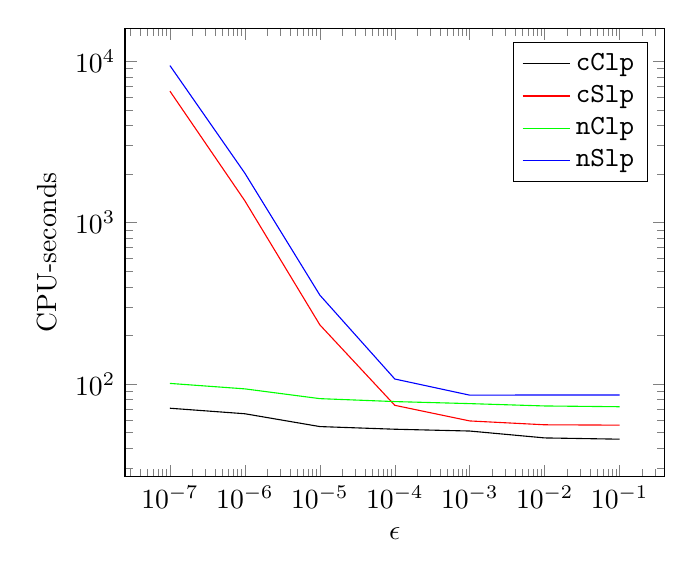
\begin{tikzpicture}
    \begin{loglogaxis}[
        xlabel=$\epsilon$,
        ylabel=CPU-seconds,
        legend pos=north east]

        \addplot[black] plot coordinates {
(0.1,       45.51)
(0.01,      46.34)
(0.001,     51.12)
(0.0001,    52.46)
(0.00001,   54.48)
(0.000001,  65.42)
(0.0000001, 70.78)
        };

        \addplot[red] plot coordinates {
(0.1,       55.61)
(0.01,      55.89)
(0.001,     59.04)
(0.0001,    73.79)
(0.00001,   232.53)
(0.000001,  1363.46)
(0.0000001, 6522.91)
        };

        \addplot[green] plot coordinates {
(0.1,       72.32)
(0.01,      73.11)
(0.001,     75.60)
(0.0001,    77.83)
(0.00001,   81.16)
(0.000001,  93.29)
(0.0000001, 100.85)
        };

        \addplot[blue] plot coordinates {
(0.1,       85.51)
(0.01,      85.51)
(0.001,     85.28)
(0.0001,    107.39)
(0.00001,   355.47)
(0.000001,  2022.25)
(0.0000001, 9395.92)
        };

        \legend{\texttt{cClp}, \texttt{cSlp}, \texttt{nClp}, \texttt{nSlp}}
    \end{loglogaxis}
\end{tikzpicture}
